\documentclass[conference]{IEEEtran}
\IEEEoverridecommandlockouts
% The preceding line is only needed to identify funding in the first footnote. If that is unneeded, please comment it out.
%Template version as of 6/27/2024

\usepackage{cite}
\usepackage{amsmath,amssymb,amsfonts}
\usepackage{algorithmic}
\usepackage{graphicx}
\usepackage{textcomp}
\usepackage{xcolor}
\usepackage{placeins}

\usepackage{tikz}
\usetikzlibrary{calc, patterns, patterns.meta, shapes.geometric, arrows.meta, positioning, fit}

\usepackage{ifthen}

\usepackage{siunitx} 
\sisetup{locale = US}
\DeclareSIUnit{\Bit}{Bit}

\usepackage{cuted}
\usepackage{stfloats}
\usepackage{tabularray}
\usepackage{matlab-prettifier}

\def\BibTeX{{\rm B\kern-.05em{\sc i\kern-.025em b}\kern-.08em
    T\kern-.1667em\lower.7ex\hbox{E}\kern-.125emX}}

\begin{document}
\title{Decoding the Amplitude-Modulated Part the DCF77 Longwave Time Signal by using the Goertzel Algorithm}

\author{\IEEEauthorblockN{1\textsuperscript{st} Leander Hackmann}
\IEEEauthorblockA{\textit{Master Embedded Systems Engineering} \\
\textit{FH Dortmund}\\
Dortmund, Germany \\
Mat.-Nr.: 7217912, leander.hackmann001@stud.fh-dortmund.de}
}

\maketitle

\begin{abstract}
    The DCF77, a long wave time signal transmitter that is located near Frankfurt am Main in Germany, is the primary source of time information for
    radio-controlled clocks in Europe. Its signal consists of a phase and an amplitude-modulated part, both containing the time information.
    Devices that use the signal usually consist of an amplitude modulation long wave receiver, often realized by using a dedicated integrated circuit, and an
    application processor. In this paper, an alternative approach for the demodulation of the amplitude-modulated part of the signal, without the need for specialized
    analog cicruitry and only a minimal amount of simple hardware components, is presented.
    This is done by utilizing direct-sampling software-defined radio techniques together with leveraging the efficiency of the Goertzel algorithm.
    As a result, the presented approach removes the need for most of the usually employed analog circuitry, leaving only a front-end amplifier, and therefore
    effectively proposes a new type of design where the receiver is implemented inside the application processor.
    The employed lightweight algorithms keep it realizable on a system with limited resources, which is shown in an example implementation on a Arm Cortex-M3 microcontroller. 
\end{abstract}

\begin{IEEEkeywords}
    DCF77, Goertzel, Digital Signal Processing, Time Signal, Software Defined Radio
\end{IEEEkeywords}

\section{Introduction}
Radio controlled clocks are very popular because they dont require periodical re-adjustment in comparison to common mechanical or quartz-powered clocks.
Instead, the information about the current time is obtained from a RF-signal that is transmitted by an official authority that ensures its availability and
correctness.
The probably most important time signal in Europe is transmitted by the station DCF77 from Mainflingen, a city in Germany that is close to Frankfurt am Main.
The station is operated by a private company that is commissioned by the Physikalisch-Technische Bundesanstalt (PTB) which also supplies the current time information,
generated by two caesium clocks and two caesium fountains. Its operating frequency lies in the long wave area at \SI{77.5}{\kilo\hertz} and the time signal
uses simple modulation techniques (amplitude and phase-modulation) and transmits with \SI{100}{\kilo\watt} Effective Isotropic Radiated Power (EIRP) to enable the reception of the
signal in relatively close distances (up to \SI{2000}{\kilo\meter}) with simple technical equipment \cite{b2}.
\begin{figure}[!htbp]
    \centerline{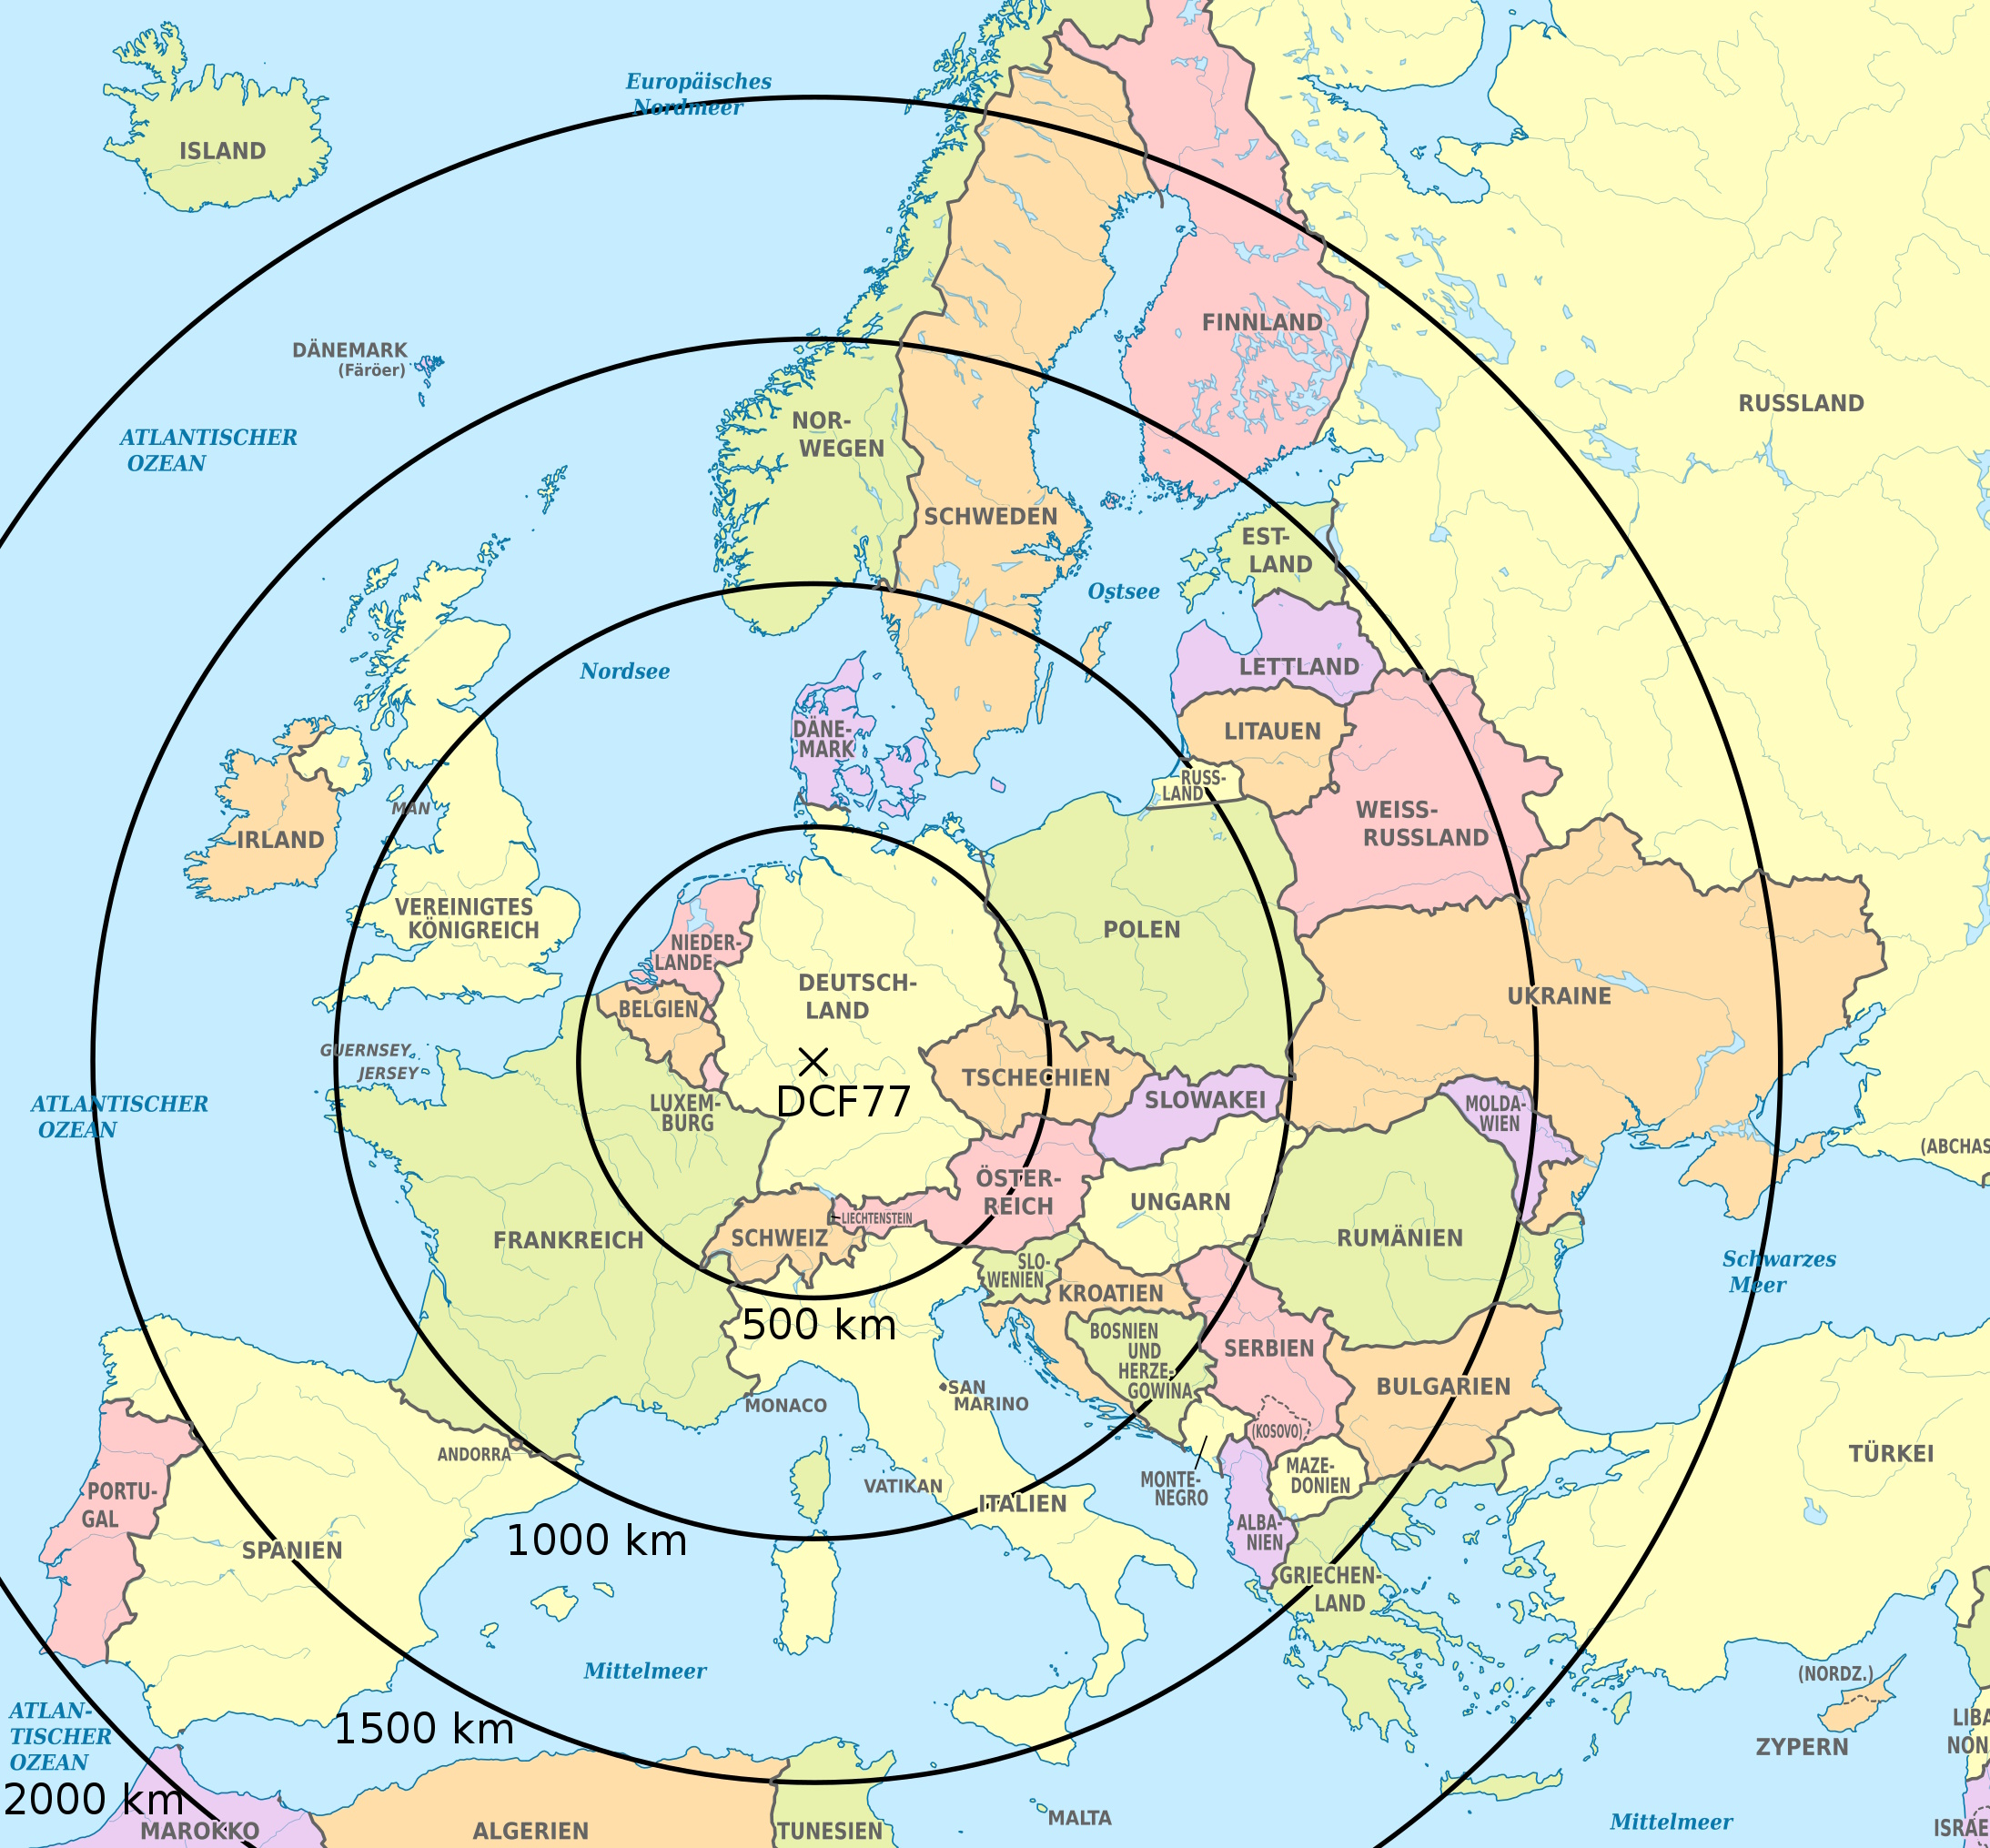
\includegraphics[width=0.3\textwidth]{img/dcf77_range.jpg}}
    \caption{Coverage of the DCF77 signal. Adapted from \cite{b1}}
    \label{fig:dcf77_range}
\end{figure}
\FloatBarrier
End-user devices usually make use of the amplitude-modulated part of the signal by using an amplitude modulation receiver, often a by employing specialized integrated circuit,
together with a rather big ferrite-rod antenna to obtain the time signal.
This time signal then needs further hardware, often in form of a microcontroller used as the applicaton processor, to decode and retrieve the actual time information.
With the increasing availability of computation power and Digital Signal Processing (DSP) capabilities inside cheap mixed-signal microcontrollers, which are already used
to process the time information, the idea to replace to replace the analog receiver portion with a Software Defined Radio (SDR) is more or less obvious.
Moving the receiver into the application processor would allow for a simpler hardware design by shrinking down the complexity and the parts count of the
external analog circuitry. In fact, only a tuned antenna with a basic pre-amplifier is needed.

In this paper, a straightfoward principle for designing a lightweight receiver for the DCF77, based on SDR-techniques, is presented.
After taking a look at the structure of the DCF77 signal, the theoretical operation principle of the receiver is explained and shown in a MATLAB simulation.
To further underline the simplicity and the possibility to implement the principle on a system with limited resources, a demonstration on a Arm Cortex-M3 microcontroller
is shown.

\section{The DCF77 signal}
The DCF77 station operates in the long wave area at a frequency of \SI{77.5}{\kilo\hertz}.
Its operation started with transmitting a frequency standard in 1959.
In 1973, the transmission of the current time information was added to the signal by using amplitude modulation.
To allow a reception under more challenging conditions and with a higher resolution and accuracy, the same time information is also added to the signal since 1983 by using
phase-modulation \cite{b3}.
The two different parts of the signal that result out of the parallel amplitude and the phase-modulation can be used for different use-cases that are separated by the
requirements regarding the resolution, accuracy, and the reliability of the obtained time information. 
Whereas the amplitude-modulated part is mainly used for general-purpose time application with low resolution requirements, the phase-modulated part is usually used
for specialized applications that require a higher resolution, accuracy, and reliability.
Although being considered as low in comparison to what is achievable by analyzing the phase-modulated part, the usually observed accuracy uncertainity when using the
amplitude-modulated part it is still well below \SI{1}{\second}, being \SI{100}{\milli\second} \cite{b2}.
When using the phase-modulated part, a standard deviation of \SIrange{\pm 2}{\pm 22}{\micro\second} from the atomic clock to the receving device can be observed \cite{b4}.
\par
As the amplitude-modulated part allows simplistic receiver designs through its straightfoward modulation scheme, it is used in the principle presented in this paper
and therefore a focus is put on explaining this part of the DCF77 signal. The following explainations in this paper therefore refer explicitly to the amplitude-modulated part.
The time information, represented as a series of binary symbols, is modulated onto the carrier with a frequency of \SI{77.5}{\kilo\hertz} by using
Amplitude-Shift Keying (ASK). Every symbol has the duration of exactly \SI{1}{\second}, with a part that is either \SI{100}{\milli\second} or \SI{200}{\milli\second}
long where it has a value equal to 0.
This the duration of this "gap" is used to encode respectively a 0 or a 1 and effectively switches the strength of the carrier between \SI{15}{\percent} and \SI{100}{\percent} \cite{b5}.
\begin{figure}[htbp]
    \centerline{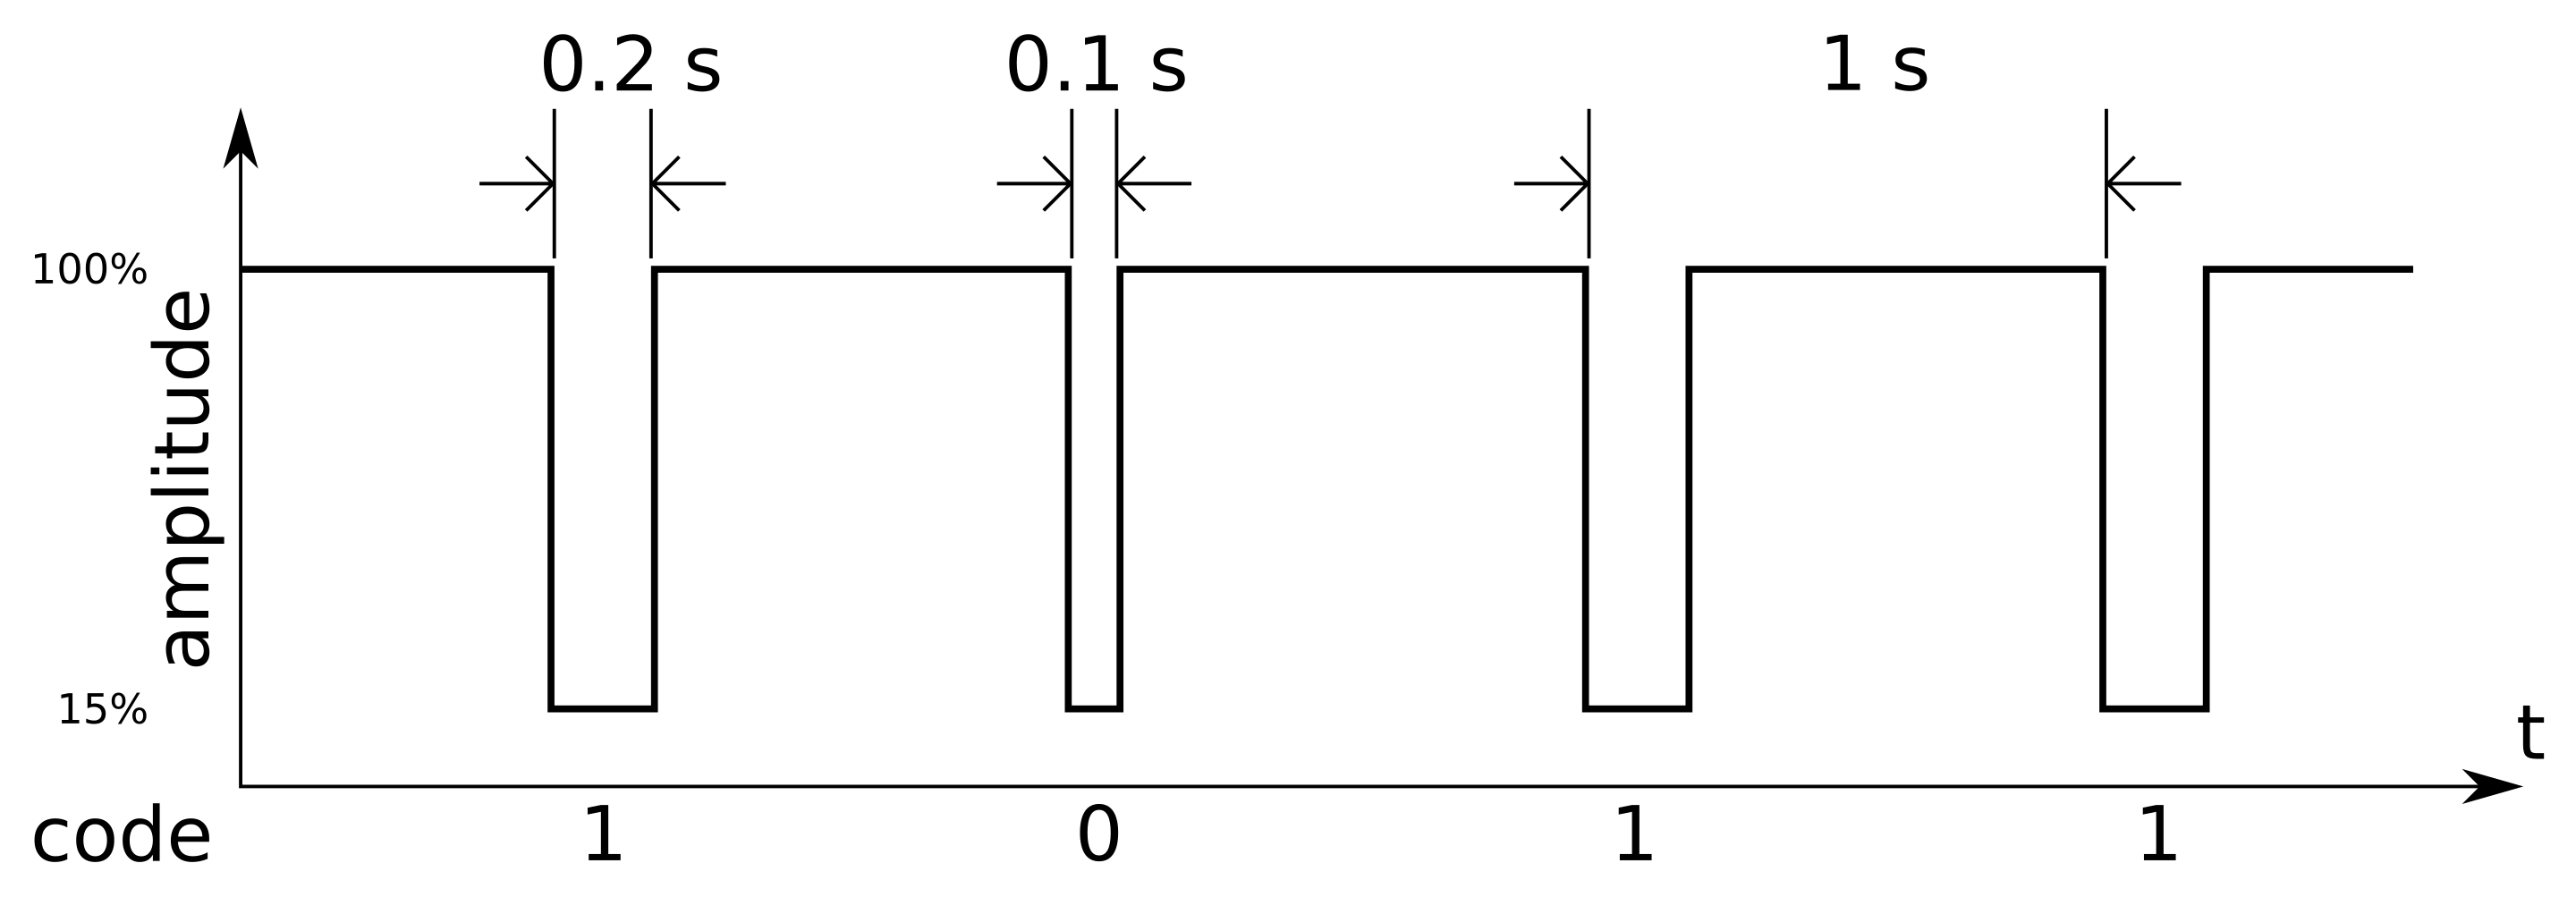
\includegraphics[width=0.45\textwidth]{img/dcf77_symbol_encoding.png}}
    \caption{Symbol encoding of the DCF77 signal. From \cite{b1}}
    \label{fig:dcf77_symbol_encoding}
\end{figure}
\FloatBarrier\noindent
To allow the detection of a new minute, the gap is left out between the last (59) second of the ongoing and the first (0) second of the next minute.
By using this scheme, a dataframe consisting out \SI{59}{\Bit}, starting at second 1, can be transmitted every minute.
Bit \SIrange{0}{19}{} are used to send encrypted weather data, to notify the PTB in case of errors in the transmitter, to announce an upcoming
switch to or from Daylight Saving Time (DST), to show if DST is currently enabled or not, and to announce an upcoming leap second \cite{b5}.
As the decryption of the weather date requires a specialized third-party integrated circuit and the notification bit is only important for the PTB, these parts
of the frame are discarded by most applications.
The leftover Bits \SIrange{20}{58}{} are used to represent the current time and date in Binary Coded Decimal (BCD) format, including parity bits for recognizing errors.
\begin{figure}[htbp]
    \centerline{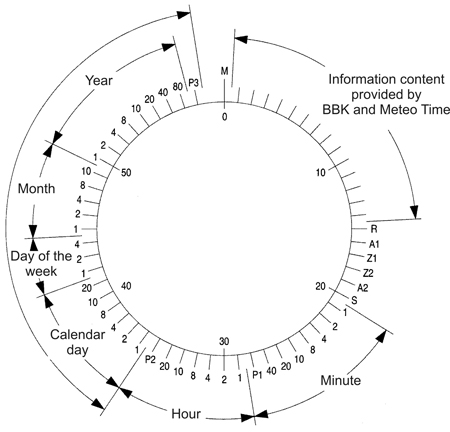
\includegraphics[width=0.35\textwidth]{img/dcf77_frame_encoding.jpg}}
    \caption{Data frame encoding of the DCF77 signal. From \cite{b5}}
    \label{fig:dcf77_data_encoding}
\end{figure}
\FloatBarrier\noindent
This means that a receiver needs to run at least for \SI{39}{\second} after powerup to receive one whole block containing the current time information.
In reality, this period is usually longer because the receiver needs to adapt to the current receiving conditions. 
These conditions underly a lot of influences, including temporary fading, electromagnetic noise from the close environment or varying signal strengths
during different times of the day.

\section{Principle of the receiver}
As the seen in the description of the DCF77 signal, retrieving back the binary time signal from the amplitude-modulated part is more or less trivial.
Conventional applications execute this task by using analog receiving circuits, usually by using a simple amplitude modulation receiver together with a
tuned ferrite-rod antenna, acting as a Bandpass Filter (BPF), to filter out the irrelevant part of the spectrum. 
Moving the receiver into the digital domain allows for more advanced techniques to retrieve this binary time signal, rather than demodulating the signal with a
diode detector inside the amplitude modulation receiver.
Because the information is contained only in the amplitude of the signal, and therefore inside the signal strength at the receiver, it can also be obtained by doing a
continuous analysis of the spectrum at the carrier's frequency of \SI{77.5}{\kilo\hertz}.
This task will be carried out by using the Goertzel algorithm, which is presented later.
The structure of the whole receiver then simplifies to only two external hardware parts
(besides the application processor) and four internal software parts.

\begin{figure}[!htbp]
    \centering
    \resizebox{0.48\textwidth}{!}{
        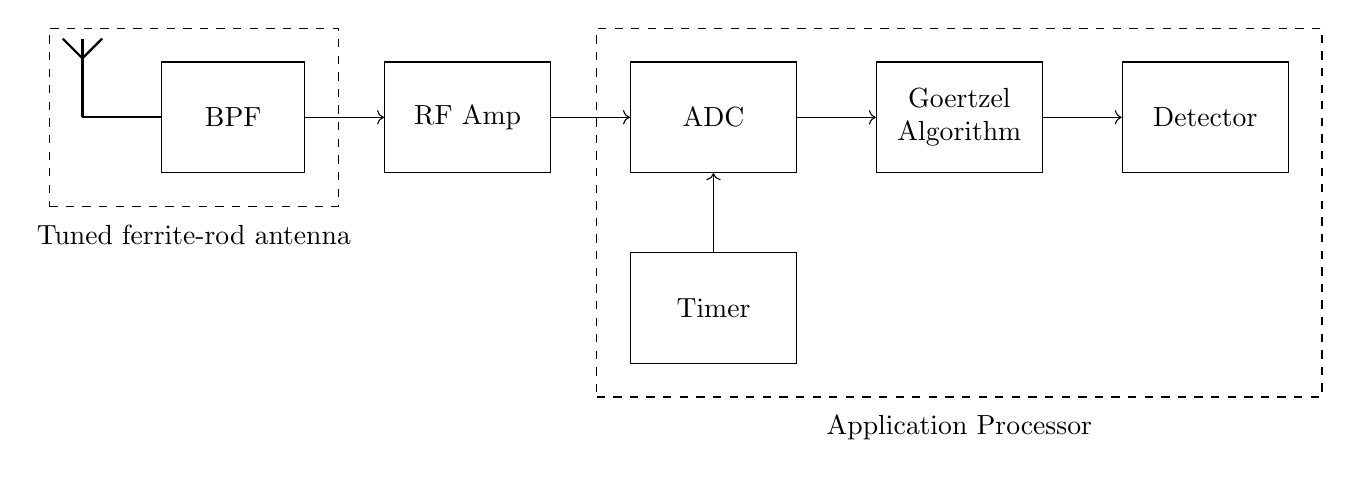
\begin{tikzpicture}
            % Block styles
            \tikzstyle{block} = [rectangle, draw, text width=4.5em, text centered, minimum width=6em, minimum height=4em]
            \tikzstyle{block_dashed} = [rectangle, draw, text width=2em, text centered, minimum width=4em, minimum height=4em, dashed]
            % Input and output
            \begin{scope}[shift={(-3,0)}] % Adjust the position of the antenna
                \coordinate (antenna) at (0,0);
                \draw[thick] (0,0) -- (0,1); % Antenna pole
                \draw[thick] (-0.25,1) -- (0,0.75); % Antenna horizontal line
                \draw[thick] (0.25,1) -- (0,0.75); % Antenna horizontal line
            \end{scope}
            \node[block, right=of antenna, minimum width=4em, minimum height=4em] (bpf) {BPF};
            \node[block, right=of bpf] (rfamp) {RF Amp};
            \node[block, right=of rfamp] (adc) {ADC};
            \node[block, below=of adc] (timer) {Timer};
            \node[block, right=of adc] (goertzel) {Goertzel Algorithm};
            \node[block, right=of goertzel] (det) {Detector};
            % Connections
            \draw[thick] (antenna) -- (bpf);
            \draw[->] (bpf) -- (rfamp); % Connection from antenna to RF amplifier
            \draw[->] (rfamp) -- (adc);
            \draw[->] (timer) -- (adc);
            \draw[->] (adc) -- (goertzel);
            \draw[->] (goertzel) -- (det);

            \node[draw, dashed, fit={(antenna) (bpf)}, inner sep=12pt] (tank_circuit) {};
            \node[below=0.3em of tank_circuit, align=center] {Tuned ferrite-rod antenna};

            \node[draw, dashed, fit={(adc) (timer) (goertzel) (det)}, inner sep=12pt] (microcontroller) {};
            \node[below=0.3em of microcontroller, align=center] {Application Processor};
        \end{tikzpicture}
    }
    \caption{Block diagram of the receiver}
    \label{fig:block_diag_receiver}
\end{figure}
\FloatBarrier\noindent
The tuned ferrite-rod antenna is kept to filter out the irrelevant spectral components, leaving only the DCF77's component at \SI{77.5}{\kilo\hertz}.
This signal is then amplified by a RF amplifier and sampled at a certain sampling rate $f_{s}$ using the Analog to Digital Converter (ADC) of the application processsor.
A timer producing a frequency equal to $f_{s}$ is used to trigger the sampling.
The samples are passed to the Goertzel algorithm to analyze the amplitude of the DCF77 signal.
The result of the analyzation is then passed to a detector to reconstruct the binary time signal.
\par
Before discussing the simulation of the whole reciever, the internal parts executing the sampling, the spectral analysis and the detection are explained in more detail,
as they use some special techniques that should be introduced and explained beforehand.

\subsection{Bandpass sampling the DCF77 signal}
Lowpass sampling is probably the most commonly used sampling technique.
Stated by the Nyquist criterion, it requires the sampling rate $f_{s}$ to be at greater or equal to twice of the frequency of the highest frequency $f_{h}$ component in the
signal to be sampled:
\begin{equation}
    f_{s} \geq 2 \cdot f_{h}
\end{equation}
Only when this condition is satisfied, the original signal can be reconstructed from the samples and it must be ensured that the signal contains no spectral elements
that might violate the condition \cite{b6}.
This is usually done by filtering the signal through a lowpass before sampling.
\par
Besides lowpass sampling, a signal can also be bandpass sampled if it is has a limited bandwidth $B$, defined by the frequency of the lowest spectral component $f_{l}$ and
the highest spectral component $f_{h}$:
\begin{equation}
    B = f_{h} - f_{l}
\end{equation}
The center frequency $f_{c}$ is then located in the middle between $f_{l}$ and $f_{h}$:
\begin{equation}
    f_{c} = \frac{f_{l} + f_{h}}{2} = f_{l} + \frac{B}{2}
\end{equation}
Signals that fulfill these requirements can also be sampled with a lower $f_{s}$ and still be reconstructed, if special care is taken when selecting the actual value of $f_{s}$.
The ranges of possible values for $f_{s}$ are defined by the conditions
\begin{equation}
    \frac{2 \cdot f_{c} - B}{m} \geq f_{s} \geq \frac{2 \cdot f_{c} + B}{m + 1} \label{eqn:fs}
\end{equation}
and
\begin{equation}
    f_{s} \geq 2 \cdot B \label{eqn:fs_b}
\end{equation}
with $m$ being an arbitrary, positive integer \cite{b6}.
During this sampling process, the signal is also shifted in frequency. This can be imagined
by a sum of convolutions of the initial spectrum with dirac delta functions, located at
positive and negative integer multiples of $f_{s}$ \cite{b9}.
\par
As the DCF77's signal fulfills the stated requirements after it is received by the tuned ferrite-rod antenna and therefore bandpass filtered, it qualifies for being bandpass sampled.
Its center frequency $f_{c}$ lies at \SI{77.5}{\kilo\hertz} with a theoretical maximum bandwidth $B$ of \SI{2.4}{\kilo\hertz} \cite{b2}.
The effective bandwidth is much smaller in reality but \SI{2.4}{\kilo\hertz} will be used for finding a proper sampling frequency to provide enough safety margin.
With \eqref{eqn:fs}, a table containing possible ranges for $f_{s}$ can be created.
\begin{table}[htbp]
    \caption{Possible ranges for $f_{s}$ with $f_{c} = \SI{77.5}{\kilo\hertz}$ and $B = \SI{2.4}{\kilo\hertz}$}
    \centering
    \begin{tblr}{|c|c|c|}
        \hline
        & Lower boundary of $f_{s}$ & Upper boundary of $f_{s}$\\
        $m$ & $\left\lceil\frac{2 \cdot f_{c} + B}{m + 1}\right\rceil$ & $\left\lfloor\frac{2 \cdot f_{c} - B}{m}\right\rfloor$\\
        \hline
        $1$ & $\SI{78700}{\hertz}$ & $\SI{152600}{\hertz}$\\
        $3$ & $\SI{52467}{\hertz}$ & $\SI{76300}{\hertz}$\\
        $4$ & $\SI{39350}{\hertz}$ & $\SI{50866}{\hertz}$\\
        $5$ & $\SI{31480}{\hertz}$ & $\SI{38150}{\hertz}$\\
        $6$ & $\SI{26234}{\hertz}$ & $\SI{30520}{\hertz}$\\
        $7$ & $\SI{22486}{\hertz}$ & $\SI{25433}{\hertz}$\\
        $8$ & $\SI{19675}{\hertz}$ & $\SI{21800}{\hertz}$\\
        $\vdots$ & $\vdots$ & $\vdots$\\
        $31$ & $\SI{4919}{\hertz}$ & $\SI{4922}{\hertz}$\\
        \color{red} $32$ & \color{red} $\SI{4770}{\hertz}$ & \color{red} $\SI{4768}{\hertz}$\\
        \color{red} $33$ & \color{red} $\SI{4630}{\hertz}$ & \color{red} $\SI{4624}{\hertz}$\\
        \hline
    \end{tblr}
    \label{tab0}
\end{table}
\FloatBarrier\noindent
It is visible that with increasing values for $m$, the value of $f_{s}$ and also the distance between the lower and the upper boundaries are decreasing.
At $m = 32$, the condition of \eqref{eqn:fs_b} is violated and at $m = 32$ the condition of \eqref{eqn:fs}, making $m = 31$ the last valid range.
Choosing a sampling rate can now be done with this table.
\par
A lower sampling rate effectively shrinks the requirements regarding computational power, memory size and the ADC's speed, but simultaneously decreases the
distance between the lower and the upper limits of the sampling rate.
This then leads to higher requirements regarding the adherence to the exact sampling rate.
A choice providing a good tradeoff between these effects $f_{s} = \SI{24}{\kilo\hertz}$ at $m = 7$, because it offers a distance of $\SI{2647}{\hertz}$ between the upper and lower limits with the sampling frequency lying almost in the middle \cite{b10}.
The DCF77 signal is then, as visible in Fig. \ref{fig:dcf77_bp_spectrum}, downconverted and centered at
\begin{equation}
    f_{c}^{'} = f_{c} - 3 \cdot f_{s} = \SI{77.5}{\kilo\hertz} - 3 \cdot \SI{24}{\kilo\hertz} = \SI{5.5}{\kilo\hertz}
\end{equation}
caused by the convolution of the initial spectrum with the dirac delta impulse located at $-3 \cdot f_{s}$. 
The following block, the Goertzel algorithm, therefore needs to analyze the spectral component at $f_{c}^{'} = \SI{5.5}{\kilo\hertz}$.

%Needs to be placed here so it is in the left column and then on the bottom of the page
\begin{figure*}[t]
    \centering
    \resizebox{0.95\textwidth}{!}{
        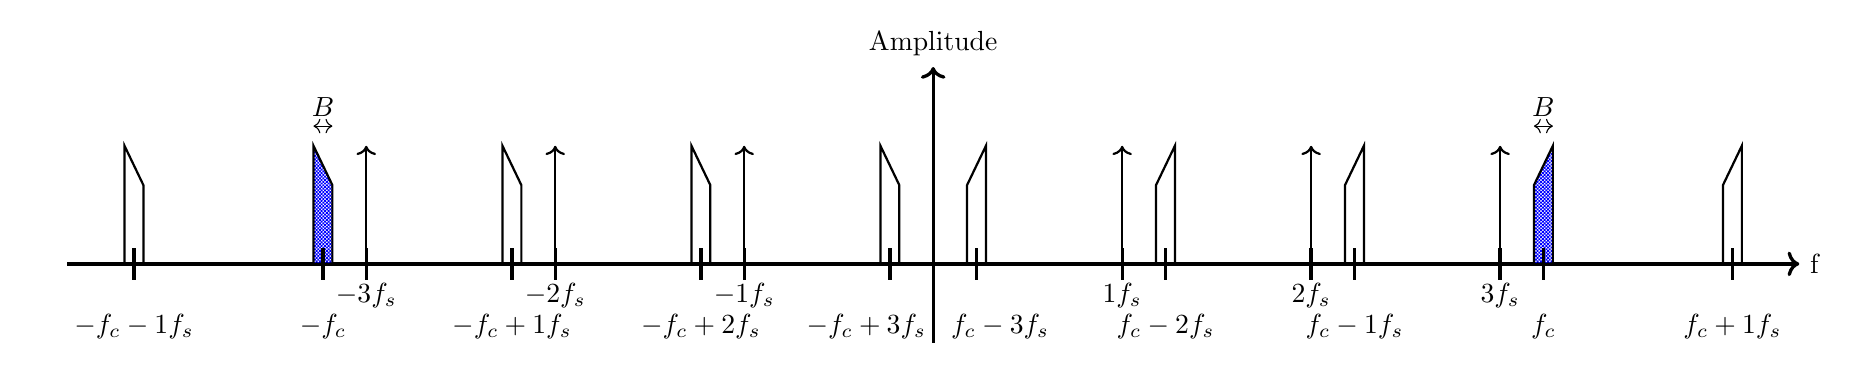
\begin{tikzpicture}
            \clip (-11.5,-1) rectangle + (23,4); %Clipping: where to start, shape and size
            
            \coordinate (fc) at (7.75,0);
            \coordinate (fs) at (2.4,0);
            
            %Axes
            \draw[->, very thick] (-11,0) -- (11,0) node[right] {f};
            \draw[->, very thick] (0,-1) -- (0,2.5) node[above] {Amplitude};
            
            %DCF77 at f_c
            \draw[thick, pattern={Dots[angle=45,distance={1.25pt/sqrt(2)}]}, pattern color=blue]
            ($(fc) + (-0.12,0)$) -- % Left line start
            ++(0,1) -- %Left line up
            ++(0.24,0.5) -- %Roof
            ++(0,-1.5) -- %Right line down
            cycle; % Close the shape
            \draw[very thick] ($(fc) + (0, -0.2)$) -- ++(0, 0.4); %Line x-axis
            \node at ($(fc) + (0, -0.8)$) {$f_{c}$}; %Index x-axis
            \draw[<->] ($(fc) + (-0.12,1.75)$) -- ++(0.24,0) node[midway, above] {$B$}; %Bandwidth

            %DCF77 at f_c
            \draw[thick, pattern={Dots[angle=45,distance={1.25pt/sqrt(2)}]}, pattern color=blue]
            ($-1*(fc) + (-0.12,0)$) -- % Left line start
            ++(0,1.5) -- %Left line up
            ++(0.24,-0.5) -- %Roof
            ++(0,-1) -- %Right line down
            cycle; % Close the shape
            \draw[very thick] ($-1*(fc) + (0, -0.2)$) -- ++(0, 0.4); %Line x-axis
            \node at ($-1*(fc) + (0, -0.8)$) {$-f_{c}$}; %Index x-axis
            \draw[<->] ($-1*(fc) + (-0.12,1.75)$) -- ++(0.24,0) node[midway, above] {$B$}; %Bandwidth

            %f_s their result of the convulutions
            \foreach \x in {-3,-2,-1,1,2,3}{
                \draw[-> , thick] ($\x*(fs)$) -- ++(0,1.5);
                \draw[very thick] ($\x*(fs) + (0,-0.2)$) -- ++(0,0.4);
                \node at ($\x*(fs) + (0,-0.4)$) {$\x f_{s}$};
                
                
                \draw[thick]
                ($(fc) + (-0.12,0) + \x*(fs)$) -- % Left line start
                ++(0,1) -- %Left line up
                ++(0.24,0.5) -- %Roof
                ++(0,-1.5) -- %Right line down
                cycle; % Close the shape
                \draw[very thick] ($(fc) + (0, -0.2) + \x*(fs)$) -- ++(0, 0.4); %Line x-axis
                \ifthenelse{\x = -3}{
                    \node at ($(fc) + (0.3, -0.8) + \x*(fs)$) {$f_{c} \pgfmathprintnumber[print sign]{\x} f_{s}$}; %Index x-axis
                }{
                    \node at ($(fc) + (0, -0.8) + \x*(fs)$) {$f_{c} \pgfmathprintnumber[print sign]{\x} f_{s}$}; %Index x-axis
                }
        
                %DCF77 at -f_c
                \draw[thick]
                ($-1*(fc) + (-0.12,0) + \x*(fs)$) -- % Left line start
                ++(0,1.5) -- %Left line up
                ++(0.24,-0.5) -- %Roof
                ++(0,-1) -- %Right line down
                cycle; % Close the shape
                \draw[very thick] ($-1*(fc) + (0, -0.2) + \x*(fs)$) -- ++(0, 0.4); %Line x-axis
                \ifthenelse{\x = 3}{
                    \node at ($-1*(fc) + (-0.3, -0.8) + \x*(fs)$) {$-f_{c} \pgfmathprintnumber[print sign]{\x} f_{s}$}; %Index x-axis
                }{
                    \node at ($-1*(fc) + (0, -0.8) + \x*(fs)$) {$-f_{c} \pgfmathprintnumber[print sign]{\x} f_{s}$}; %Index x-axis
                }
            };
        \end{tikzpicture}
    }
    \caption{Spectrum after bandpass sampling the DCF77 signal at $f_{s} = \SI{24}{\kilo\hertz}$. The original spectral parts are filled with blue dots.}
    \label{fig:dcf77_bp_spectrum}
\end{figure*}

\subsection{The Goertzel Algorithm}
The standard approach to analyze a spectrum in the digital domain after sampling is the well-known Discrete Fourier Transform (DFT), implemented by using
the Fast Fourier Transform (FFT). This yields an analysis of the complete spectrum, producing $\frac{N}{2} + 1$ relevant results for equally distributed frequencies
("frequency bins") within a range from \SI{0}{\hertz} to $\frac{f_{s}}{2}$ where $N$ is the number of samples and $f_{s}$ is the sampling frequency \cite{b6}.
The signal strength, and therefore the binary time signal of the amplitude-modulated part, can then be examined by observing the magnitude of the curresponding frequency bin
over time. Because of only one frequency bin being relevant, it is obvious that a full FFT produces a lot of overhead and redundant calculation operations in this use-case. 
This overhead can be avoided by using the Goertzel algorithm instead of the FFT, which is able to calculate the value of one specific frequency bin with a smaller
amount of needed calculations.
It was invented in 1958 by Gerald Goertzel and since then is most commonly used in the detection of tones employed in Dual-tone Multi-frequency (DTMF) signaling \cite{b7}.
The working principle of the algorithm can be percieved as a second-order Infinite Impulse Response (IIR) filter (see \eqref{eqn:goertzel}) where the results $y[n-1]$ and $y[n-2]$ of the output $y[n]$
are stored in the states $Q_{1}$ and $Q_{2}$, so they are still available after the execution of the filter \cite{b8}.
\begin{equation}
    y[n] = x[n] + 2 \cdot cos(\omega_{g}) \cdot y[n-1] - y[n-2]
    \label{eqn:goertzel}
\end{equation}
\begin{figure}[h]
    \centering
    \resizebox{0.4\textwidth}{!}{
        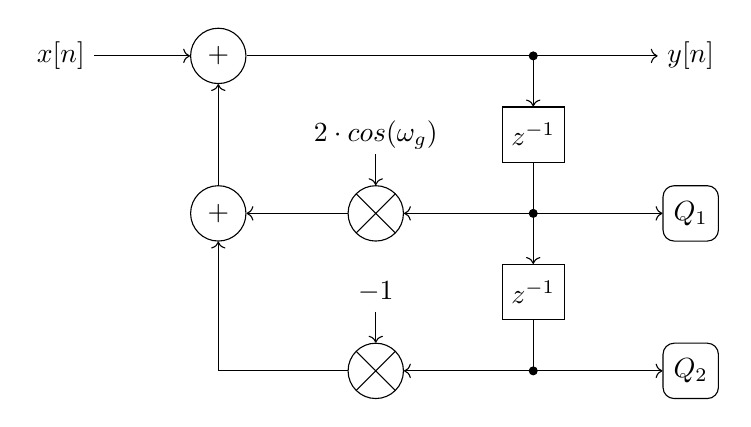
\begin{tikzpicture}[auto, node distance=2cm]
            %Defining a cross set for the multiplication elements
            \tikzset{cross/.style={path picture={ 
            \draw[black]
            (path picture bounding box.south east) -- (path picture bounding box.north west) (path picture bounding box.south west) -- (path picture bounding box.north east);
            }}}
          
          % Define block styles
            \tikzstyle{delay} = [draw, rectangle, minimum height=2em, minimum width=2em]
            \tikzstyle{sum} = [draw, circle, minimum size=2em, node distance=1.5cm]
            \tikzstyle{mult} = [draw, circle, minimum size=2em, node distance=1.5cm, cross]
            \tikzstyle{state} = [draw, rectangle, rounded corners, minimum height=2em, minimum width=2em]
            
            % Nodes
            \node at (-2, 0) (x) {$x[n]$};
            \node[sum] at (0,0) (sum1) {+};
            \node[sum] at (0,-2) (sum2) {+};
            \node[mult] at (2,-2) (mult1) {};
            \node[mult] at (2,-4) (mult2) {};
            \node[delay] at (4,-1) (del1) {$z^{-1}$};
            \node[delay] at (4,-3) (del2) {$z^{-1}$};
            \node[state] at (6,-2) (st1) {$Q_{1}$};
            \node[state] at (6,-4) (st2) {$Q_{2}$};
            \node at (6, 0) (y) {$y[n]$};

            \draw[->] (x.east) -- (sum1.west);
            \draw[->] (sum1.east) -- (y.west);
            \draw[->] (sum2.north) -- (sum1.south);
            \draw[->] (mult1.west) -- (sum2.east);
            \draw[->] (mult2.west) -- (0, -4) -- (sum2.south);
            \draw[->] (4, 0) -- (del1.north);
            \draw[->] (del1.south) -- (del2.north);
            \draw[->] (del2.south) -- (4,-4) -- (mult2.east);
            \draw[->] (4,-2) -- (mult1.east);
            \draw[->] (2, -1.25) -- (mult1.north);
            \draw[->] (2, -3.25) -- (mult2.north);
            \draw[->] (4, -2) -- (st1.west);
            \draw[->] (4, -4) -- (st2.west);
            \node at (2, -1) {$2 \cdot cos(\omega_{g})$};
            \node at (2, -3) {$-1$};
            \node[draw, shape=circle, fill=black, scale=0.3] at (4,0) {};
            \node[draw, shape=circle, fill=black, scale=0.3] at (4,-2) {};
            \node[draw, shape=circle, fill=black, scale=0.3] at (4,-4) {};
        \end{tikzpicture}
    }
    \caption{Block diagram of the Goertzel algorithm without the final calculation of the squared magnitude}
    \label{fig:goertzel_iir}
\end{figure}
\FloatBarrier\noindent
The system takes the input sequence $x[n]$ with length $N$ and is executed exactly $N$ times.
After the execution, the squared magnitude of $f_{a}$, the frequency to be analyzed inside $x[n]$, can be calculated using the values of the two states $Q_{1}$ and $Q_{2}$:
\begin{equation}
    |X(f_{a})|^2 = Q_{1}^2 + Q_{2}^2 - Q_{1} \cdot Q_{2} \cdot 2 \cdot \cos(\omega_{g})
\end{equation}
The constant $2 \cdot cos(\omega_{g})$, often called the "Goertzel coefficient", is calculated before the execution and used to adapt the algorithm to the frequency to be analyzed.
The Value of $\omega_{g}$ itself is calculated based on a integer number $k$ and $N$.
The integer number $k$ is a rounded fraction based on $N$, the frequency to be analyzed $f_{a}$, and the the sampling frequency $f_{s}$:
\begin{equation}
    k = \left\lfloor \frac{N \cdot f_{a}}{f_{s}} \right\rceil
\end{equation}
\begin{equation}
    w_g = \frac{2\pi \cdot k}{N}
\end{equation}

\par
Just as with the conventional FFT, the amount of needed calculations for executing the Goertzel algorithm is based on the number of samples.
In total, $N + 1$ multiplications and $2 \cdot N + 2$ additions are needed, which can be seen from the formulas for the IIR-part and the final calculation of the squared magnitude.
For example, a length of processing $N = 512$ samples requires in $513$ multiplications and $1026$ additions to calculate the squared magnitude of the desired frequency.
In comparison, the typical radix-2 FFT, needs $\frac{N}{2} \cdot \log_{2}(N)$ complex multiplications and $N \cdot \log_{2}(N)$ complex additions to be completed. With $N = 512$ this would result in $2034$ complex multiplications and $4608$ complex additions.
\par
With this simple example, it is already visible that the Goertzel algorithm can reduce the amount of needed resources compared to a full FFT, when only one or a small amount of frequency bins should be analyzed.
It is therefore used to observe the DCF77 signal's amplitude over time by being executed periodically.
As the gap of the encoded symbols is eiter \SI{100}{\milli\second} or \SI{200}{\milli\second} long, the duration of the analyzation set to \SI{10}{\milli\second} to provide a good tradeoff between resolution in time and a longest possible analyzation time
to leverage the DFT gain.
The square roots of the results are taken to finally calculate the magnitude of the DCF77 signal's amplitude and then passed to a detector to obtain the binary time signal.
Because of the duration of the analyzation being equal to \SI{10}{\milli\second}, the sampling rate after the Goertzel algorithm is equal to:
\begin{equation}
    f_{s,g} = \frac{1}{\SI{10}{\milli\second}} = \SI{100}{\hertz}
\end{equation}

\subsection{The detector}
The output of the Goertzel algorithm is already following the waveform of the binary time signal but still includes fluctuations due to noise and fading.
To reconstruct the original waveform of the binary time signal, it is processed inside a detector.
As the values of the Goertzel algorithm will follow the pattern of the signal's amplitude being switched between \SI{15}{\percent} and \SI{100}{\percent}, the detection can be done by comparing the value of the current sample to a threshold.
To compensate the changing of magnitude of the Goertzel algorithm's values that is caused by the current receiving situation, an Exponential Moving Average (EMA) is calculated by using \eqref{eqn:ema} and employed to create an adaptive threshold \cite{b11}.
\begin{equation}
    y[t] = \alpha \cdot x[t] + (1 - \alpha) \cdot y[t-1]
    \label{eqn:ema}
\end{equation}
This part can also be represented as a block diagram:
\begin{figure}[h]
    \centering
    \resizebox{0.4\textwidth}{!}{
        \begin{tikzpicture}[auto, node distance=2cm]
            %Defining a cross set for the multiplication elements
            \tikzset{cross/.style={path picture={ 
            \draw[black]
            (path picture bounding box.south east) -- (path picture bounding box.north west) (path picture bounding box.south west) -- (path picture bounding box.north east);
            }}}
          
            %Block styles
            \tikzstyle{delay} = [draw, rectangle, minimum height=2em, minimum width=2em]
            \tikzstyle{sum} = [draw, circle, minimum size=2em, node distance=1.5cm]
            \tikzstyle{mult} = [draw, circle, minimum size=2em, node distance=1.5cm, cross]
            \tikzstyle{state} = [draw, rectangle, rounded corners, minimum height=2em, minimum width=2em]
            
            %Nodes
            \node at (-1.5, 0) (x) {$x[n]$};
            \node[mult] at (0,0) (mult1) {};
            \node[sum] at (1.5,0) (sum1) {+};
            \node[mult] at (3,-2) (mult2) {};
            \node[delay] at (4.5,-1) (del1) {$z^{-1}$};
            \node at (6, 0) (y) {$y[n]$};

            \draw[->] (x.east) -- (mult1.west);
            \draw[->] (mult1.east) -- (sum1.west);
            \draw[->] (sum1.east) -- (y.west);
            \draw[->] (mult2.west) -- (1.5, -2) -- (sum1.south);
            \draw[->] (del1.south) -- (4.5, -2) -- (mult2.east);
            \draw[->] (4.5, 0) -- (del1.north);
            \draw[->] (0, 0.75) -- (mult1.north);
            \draw[->] (3, -1.25) -- (mult2.north);
            \node at (0, 1) {$\alpha$};
            \node at (3, -1) {$1 - \alpha$};
            \node[draw, shape=circle, fill=black, scale=0.3] at (4.5,0) {};
        \end{tikzpicture}
    }
    \caption{Block diagram showing the calculation of the EMA}
    \label{fig:ema_iir}
\end{figure}
\FloatBarrier\noindent
The value of the smoothing factor $\alpha$ was calculated to take the samples of the last \SI{10}{\second} into account:
\begin{equation}
    \begin{split}
        \alpha &= \frac{2}{N + 1} = \frac{2}{\SI{10}{\second} \cdot f_{s,g} + 1}\\
        &= \frac{2}{\SI{10}{\second} \cdot \SI{100}{\hertz} + 1} \approx 0.001998
    \end{split}
\end{equation}
This provides a stable and slowly changing average, as it is putting more weight on the past samples and leaves minimal influence to the most recent sample.
The decision is then done by comparing the current sample to a threshold calculated by multiplying the current value of the average with $0.575$ (the middle bewteen \SI{15}{\percent} and \SI{100}{\percent}) and a scaling factor of $\frac{1}{0.8725}$.
The scaling factor is needed as the average percentage of time where the signal where is equal to \SI{100}{percent} is \SI{87.25}{\percent} (assuming an equal distribution between symbols representing a binary 1 and a 0).
If the value of the current sample is above this threshold, it is treated as a 1.
Otherwise it is treated as a 0.
The series of ones and zeros is then following the waveform shown in Fig. \ref{fig:dcf77_symbol_encoding} and can be used to decode the current time. 

\section{MATLAB Simulation of the Receiver}
To verify and underline the working principle of the receiver, a simulation of the whole system was created using MATLAB.
The whole simulation was divided into five sections to allow for a clear structure:
\begin{enumerate}
    \item Simulation Parameter Section
    \item Signal Creation Section
    \item Goertzel Algorithm Section
    \item Detection Section
    \item FFT and Plot Section
\end{enumerate}
These sections will be discussed in the following.

\subsection{Simulation Parameter Section}
In the Simulation Parameter Section, static parameters for the following sections are defined.
These include the sampling frequency $f_{s}$, the duration of the whole simulation, the wanted SNR that the signal should have after passing the Additive White Gaussian Noise (AWGN)-Channel, the duration of the Goertzel algorithm segments, and the time that should
be taken into account by the EMA.
By adjusting these parameters, the behavior of the receiver can be altered to, e.g. to simulate different receiving conditions.

\subsection{Signal Creation Section}

\begin{lstlisting}[style=Matlab-editor]
    %Creating the DCF77 signal by using Amplitude Modulation (carrier is reduced to 15% during the gap)
    dcf77_signal = (0.85*time_code_signal + 0.15) .* carrier_signal;
    
    %Add noise by passing the DCF77 signal through an AWGN-Channel
    dcf77_signal_noise = awgn(dcf77_signal, awgn_snr, 'measured');
\end{lstlisting}

\section*{Acknowledgment}
The preferred spelling of the word ``acknowledgment'' in America is without 
an ``e'' after the ``g''. Avoid the stilted expression ``one of us (R. B. 
G.) thanks $\ldots$''. Instead, try ``R. B. G. thanks$\ldots$''. Put sponsor 
acknowledgments in the unnumbered footnote on the first page.


\begin{thebibliography}{00}
\bibitem{b1} -, ``DCF77,'' 2024, Wikipedia entry. [Online]. Available: https://de.wikipedia.org/wiki/DCF77
\bibitem{b2} D. Priester and P. Hetzel and A. Bauch, ``Zeit- und Normalfrequenzverbreitung mit DCF77,'' PTB Mitteilungen, 2004, [Online]. Available: https://www.ptb.de/cms/fileadmin/internet/fachabteilungen/abteilung\_4/4.4\_zeit\_und\_frequenz/4.42/dcf77.pdf
\bibitem{b3} D. Priester and P. Hetzel and A. Bauch, ``Zeit- und Normalfrequenzverbreitung mit DCF77: 1959-2009 und darüber hinaus,'' PTB Mitteilungen, 2009, [Online]. Available: https://www.ptb.de/cms/fileadmin/internet/fachabteilungen/abteilung\_4/4.4\_zeit\_und\_frequenz/pdf/2009\_Bauch\_PTBM\_\_DCF77.pdf
\bibitem{b4} P. Hetzel, ``Time dissemination via the LF transmitter DCF77 using a pseudo-random phase-shift keying of the carrier,'' PTB Braunschweig, 1988, [Online]. Available: https://www.ptb.de/cms/fileadmin/internet/fachabteilungen/abteilung\_4/4.4\_zeit\_und\_frequenz/pdf/5\_1988\_Hetzel\_-\_Proc\_EFTF\_88.pdf
\bibitem{b5} -, ``DCF77 webpage,'' 2024, Official page of the PTB [Online]. Available: https://www.ptb.de/cms/en/ptb/fachabteilungen/abt4/fb-44/ag-442/dissemination-of-legal-time/dcf77.html
\bibitem{b6} R. G. Lyons, ``Understanding Digital Signal Processing,'' Third Edition, Prentice Hall, 2010.
\bibitem{b9} J. Hoffmann, ``Sampling bandpass signals,'' 2021, Internet Article. [Online]. Available: https://www.dsprelated.com/showarticle/1407.php
\bibitem{b10} F. Zaplata and M. Kasal, ``SDR Implementation for DCF77,'', 2013, IEEE Paper. [Online]. Available: https://ieeexplore.ieee.org/document/6530943
\bibitem{b7} -, ``Goertzel algorithm,'' 2024, Wikipedia entry. [Online]. Available: https://en.wikipedia.org/wiki/Goertzel\_algorithm
\bibitem{b8} K. Banks, ``The Goertzel Algorithm,'' 2002, Internet Article. [Online]. Available: https://courses.cs.washington.edu/courses/cse466/12au/calendar/Goertzel-EETimes.pdf
\bibitem{b11} R. G. Lyons, ``Setting the 3-dB Cutoff Frequency of an Exponential Averager,'' 2012, Internet Article. [Online]. Available: https://www.dsprelated.com/showarticle/182.php
\end{thebibliography}
\end{document}